\documentclass{article}
\usepackage[utf8]{inputenc}
\usepackage[english, georgian]{babel}
\usepackage{fontspec}
\usepackage{geometry, graphicx}
\usepackage[noae]{Sweave} % you must load Sweave with the `noae` option

\setmainfont[
Extension=.ttf,
UprightFont={*},
BoldFont = {arial_geo-bold},
ItalicFont = {arial_geo-italic},
BoldItalicFont = {arial_geo-bold-italic}
]{arial_geo}

\usepackage{hyperref}
\hypersetup{
    colorlinks=true,
    linkcolor=blue,
    filecolor=magenta,      
    urlcolor=cyan,
}

\title{ლაბორატორული სამუშაო 1: შესავალი R-გარემოში}
\date{\today}

\begin{document}
\maketitle
\section*{თემები}
\begin{itemize}
\item შესავალი R-გარემოში
\item R-ის მომხმარებლის გრაფიკული გარემო: R-Studio
\item R-ის მომხმარებლის გრაფიკული გარემოს ძირითადი ელემენტები
\item R-მარკირების დოკუმენტის შექმნა
\item ,,წიგნიერი პროგრამირება'' და პროექტების ორგანიზების კარგი პრაქტიკა 
\end{itemize}

\section*{ინსტრუქცია:}

თანმიმდევრობით შეასრულეთ მითითებული ამოცანები. თქვენს $.rmd$ ფაილს სახელწოდება მიანიჭეთ შემდეგი ფორმით: თქვენი გვარი$_lab1.rmd$. მაგალითად:


\section*{დავალებები:}

\subsection*{ფაილების სისტემა და ნავიგაცია:}

პირველ რიგში, შექმენით სამუშაო დირექტორია თქვენს კომპიუტერში. რახან ამ კურსის ფარგლებში თითქმის ყოველი ლექციის შემდეგ პრაქტიკული სამუშაოა გათვალისწინებული, შექმენით კურსისთვის ცალკე ფოლდერი, სახელად $"intro_stats_r"$. ამ ფოლდერში დაამატეთ ქვე-ფოლდერი $"lab_1"$, სადაც პირველი ლაბორატორიული სამუშაოს მასალებს შეინახავთ.

\begin{figure}[h]
\centering
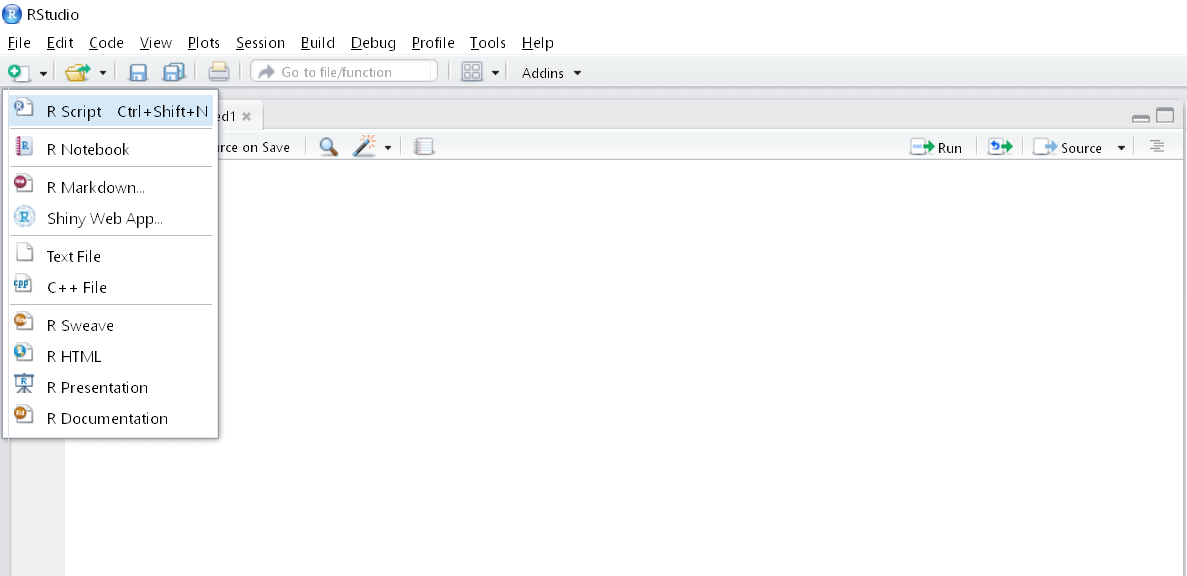
\includegraphics[width=\textwidth]{img/new_menu.PNG}
\caption{ახალი ფაილის შექმნა}
    \label{create:file}
\end{figure}

გახსენით R-Studio და შექმენით R-ბლოკნოტის ახალი ფაილი. დაარქვით სახელი და შეინახეთ $"lab_1"$ ფოლდერში. შეგახსენებთ, რომ ფაილის შექმნა შესაძლებელია მენიუს შესაბამის ელემენტზე დაწკაპუნებით და სასურველი ტიპის ფაილის არჩევით (სურ. \ref{create:file}).

<<echo=FALSE, eval=FALSE,results=tex>>=
library("xtable")
print(xtable(myData),
  floating=FALSE,
  hline.after=NULL,
  add.to.row=list(pos=list(-1,0, nrow(myData)),
  command=c('\\toprule\n','\\midrule\n','\\bottomrule\n')))
@


შესანიშნავია! ახლა ბლოკნოტის დასაწყისში, პრეამბულის შემდეგ (იხ. სურათი \ref{preamble}) აკრიფეთ მცირე ტექსტი R-studio-ზე თქვენი პირველი შთაბეჭდილებების შესახებ. ორი ან სამი წინადადება საკმარისია.

\begin{figure}[h]
\centering
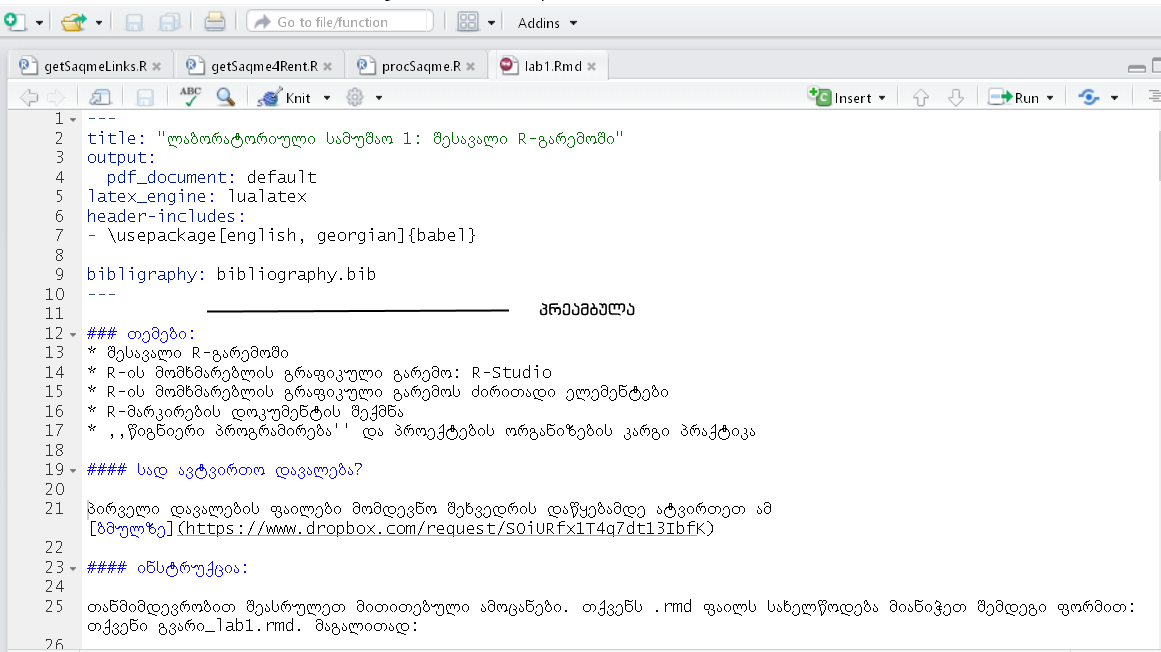
\includegraphics[width=\textwidth]{img/preamble.PNG}
\caption{დოკუმენტის პრეამბულა}
    \label{preamble}
\end{figure}

R-ბლოკნოტში ჩასვით კოდის ნაწილის აღმნიშვნელი მარკერები. დარწმუნდით, რომ თქვენი კოდი აქტიურია, რისთვისაც დააჭირეთ მარჯვენა კუთხეში მდებარე მწვანე სამკუთხა ღილაკს (იხ. სურ. \ref{chunk}). აქცენტის ნიშნებს შორის მიუთითეთ სინტაქსი, რომლის მეშვეობითაც თქვენს სამუშაო დირექტორიაში გადაინაცვლებთ.


ბიბლიოთეკების ჩამოტვირთვა და გამოძახება

R-ბლოკნოტში ჩასვით კოდის ახალი ნაწილი. ჩაწერეთ სინტაქსი, რომელიც ჩამოტვირთავს ბიბლიოთეკას ggplot2. გაუშვით სინტაქსი და დარწმუნდით, რომ იგი მუშაობს.

ახალ კოდის ნაწილში მიუთითეთ სინტაქსი, რომელიც ggplot2 ბიბლიოთეკას გაააქტიურებს. წინა დავალების მსგავსად, გაუშვით და შეამოწმეთ, ყველაფერი რიგზეა თუ არა.

\subsection*{ სკრიპტის ფაილის შექმნა და მისი ბლოკნოტში შემოტანა}

დააჭირეთ ახალი ფაილის შექმნის ღილაკს და აირჩიეთ R სკრიპტის ფაილი. გაითვალისწინეთ, რომ სკრიპში მუშაობისას, ტექსტის ჩვეულებრივად მითითება არ ხდება. თუ სიტყვიერი ახსნის ჩაწერა გჭირდებათ, მაშინ ტექსტის წინ დიეზის ნიშანი უნდა ჩაწეროთ და კოდი ,,გააკომენტაროთ'' (იხ. სურ. \ref{comment}). ასეთ კოდს პროგრამა შესრულებისას უგულებელყოფს.

\begin{figure}[h]
\centering
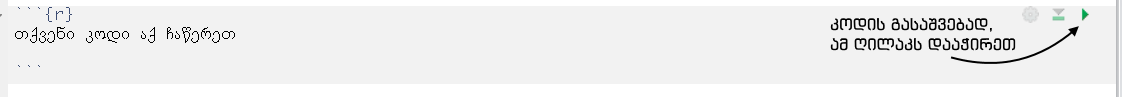
\includegraphics[width=\textwidth]{img/run_chunk.PNG}
\caption{კოდის ნაწილის მითითება და გაშვება}
    \label{chunk}
\end{figure}


სკრიპტის ფაილში ჩაწერეთ სინტაქსი, რომელიც tidyr ბიბლიოთეკას ჩამოტვირთავს და გაააქტიურებს. სკრიპტის ფაილი სამუშაო დირექტორიაში, სპეციალური ქვეფოლდერში "source" შეინახეთ და ლოგიკური სახელი მიანიჭეთ.

წიგნიერი პროგრამირების წესებით რომ ვიმოქმედოთ, საჭიროა სკრიპტის ფაილი ბლოკნოტიდან გავუშვათ. ამისთვის დაუბრუნდით ბლოკნოტს, ჩასვით ახალი კოდის ნაწილი, ჩაწერეთ სკრიპტის გასაშვები სინტაქსი და შეასრულეთ.

\subsection*{დოკუმენტის საბოლოო გაფორმება}

წიგნიერი პროგრამირების პრინციპების კიდევ ერთხელ დაცვის მიზნით, თითოეულ კოდის ნაწილს მიუწერეთ მცირე აღწერა, თუ რა ფუნქციას ასრულებს. ტექსტის გაფორმებისთვის გამოიყენეთ მარკირების ენის მრავალფეროვანი შესაძლებლობები. მაგალითად, გამოყავით სექციები, ჩასვით ბმულები, სურათები. ტექსტი გააფორმეთ კურსივით და მსხვილი ასოებით და ა. შ. მარკირების ენის დეტალური დოკუმენტაცია \href{https://www.rstudio.com/wp-content/uploads/2016/03/rmarkdown-cheatsheet-2.0.pdf}{ამ} და  \href{https://github.com/adam-p/markdown-here/wiki/Markdown-Cheatsheet}{ამ} ბმულზე შეგიძლიათ, ნახოთ.

\begin{figure}[h]
\centering
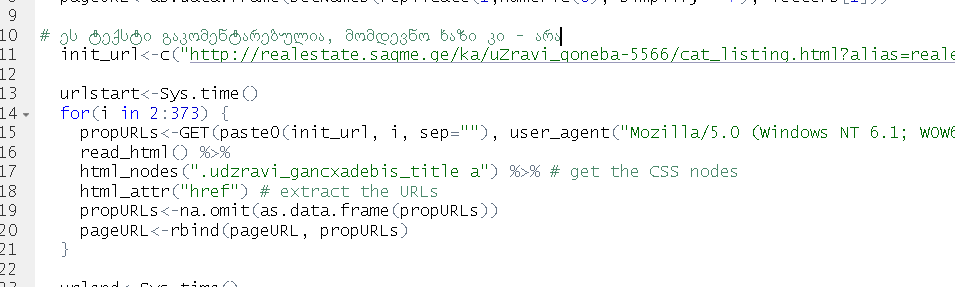
\includegraphics[width=\textwidth]{img/commented.PNG}
\caption{კოდის გაკომენტარება}
    \label{comment}
\end{figure}



\subsection*{დოკუმენტის კომპილაცია}

კომპილაციამდე (ე.ი. მარკირების html ფორმატში გადატანამდე) შეინახეთ თქვენი ბლოკნოტი. html ანუ ჰიპერტექსტების მარიკრების ენის დოკუმენტი ნებისმიერი ვებსაიტის საფუძველია - ნებისმიერი ვებგვერდი, რასაც თქვენს ბროუზერში ხედავთ, html-დოკუმენტების ერთობლიობას წარმოადგენს. R-ბლოკნოტი მარკირების შემდეგ ცალკე html-დოკუმენტად იქცევა, რომლის გახსნა ნებისმიერი, შედარებით თანამედროვე ბროუზერის მეშვეობითაა შესაძლებელი.

\begin{figure}[h]
\centering
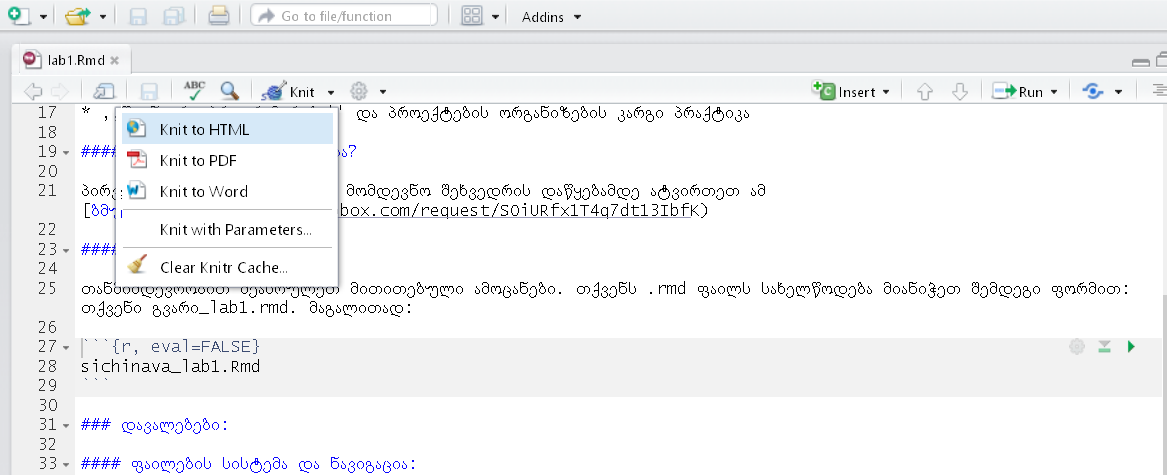
\includegraphics[width=\textwidth]{img/knit_to_html.PNG}
\caption{ბლოკნოტის კომპილაცია}
    \label{compile}
\end{figure}


ბლოკნოტის კომპილაციისთვის დააჭირეთ ძაფის გორგლის ფორმის ღილაკს და აირჩიეთ ბრძანება $knit to HTML$ (იხ. სურ. \ref{compile}. თუ ყველაფერი სწორად გააკეთეთ, მზა დოკუმენტი ავტომატურად გაიხსნება. გახსოვდეთ, რომ კომპილაციის დროს, $R-Studio$ კოდის ნაწილებში მითითებულ სინტაქსსაც ასრულებს.

\subsection*{მოვრჩი. როგორ ჩავაბარო ჩემი ნამუშევარი?}

თქვენს მიერ შექმნილი დირექტორია დააარქივეთ ($.zip$ ან $.rar$ ფორმატში). მიღებულ ფაილს სახელი დაარქვით შემდეგი ფორმატით: გვარი$_lab1.zip$. მაგალითდ:


მიღებული ფაილი მომდევნო შეხვედრის დაწყებამდე ატვირთეთ ამ \href{https://www.dropbox.com/request/SOiURfx1T4q7dt13IbfK}{ბმულზე}



\end{document}
